%\documentclass[letter]{article}
%
%\usepackage{ijcai15}
%\usepackage{times}
%
%\usepackage{eurosym}
%\usepackage{hyperref}		% clickable references
%
%\usepackage{apacite}            % APA style citations
%\usepackage{apacdoc}
%
%\usepackage{amsmath,amssymb}	% math structures and symbols
%\usepackage{graphicx}		% including of graphics files in various formats
%\usepackage{amsfonts}
%\usepackage{dialogue}
%\usepackage{placeins}
%\usepackage{tikz}
%\usetikzlibrary{positioning,backgrounds,fit,arrows,shapes,shadows}
%\usetikzlibrary{shapes.multipart}
%\usepackage{wrapfig}
%\usepackage{enumitem}
%\usepackage{framed}
%
%% \hypersetup{hidelinks}
%
%\usepackage[xspace,mla]{ellipsis}
%
%\definecolor{myyellow}{RGB}{242,226,149}
%\definecolor{mygreen}{RGB}{144,238,144}
%\definecolor{mypink}{RGB}{255,182,193}
%\definecolor{myorange}{RGB}{255,165,0}
%\definecolor{myblue}{RGB}{0,204,204}
%
%\usepackage{xparse}
%\NewDocumentCommand\StickyNote{O{4cm}mmO{4cm}}{%
%\begin{tikzpicture}
%\node[
%drop shadow={
%  shadow xshift=2pt,
%  shadow yshift=-4pt
%},
%inner xsep=7pt,
%fill=#2,
%xslant=-0.05,
%yslant=0.05,
%inner ysep=10pt
%] {\parbox[t][#1][c]{#4}{#3}};
%\end{tikzpicture}%
%}
%
%\urldef{\mailsa}\path|{j.corneli,s.colton}@gold.ac.uk|
%\urldef{\mailsb}\path|a.pease@dundee.co.uk|
%
%\newcommand{\Fw}{{\sf FloWr}}
%\newcommand{\dec}[1]{\raisebox{.2ex}{$\star$}#1\raisebox{.2ex}{$\star$}}
%
%\newcommand{\keywords}[1]{\par\addvspace\baselineskip
%\noindent\keywordname\enspace\ignorespaces#1}
%
%\begin{document}
%
%% TITLE INFORMATION
%\title{Implementing feedback in creative systems}
%
%\author{Joseph Corneli\textsuperscript{1} and Anna Jordanous\textsuperscript{2}\\
%\textsuperscript{1} Department of Computing, Goldsmiths College, University of London\\
%\textsuperscript{2} School of Computing, University of Kent}
%
%\date{today}
%
%\maketitle
%
%\begin{abstract} 
%% First attempt
%%% Various social strategies, ranging from Writers Workshops to open
%%% source software, pair programming, and design charettes have been
%%% developed to exploit emergent effects and to develop new shared
%%% language.  We investigate the feasibility of using designs of this
%%% sort in multi-agent systems that learn by sharing and discussing
%%% partial understandings.  Building on earlier theoretical work, we
%%% describe concrete implementation plans and some preliminary results.
%\end{abstract}
%
%% END OF COMMENTED OUT PART



\section{Implementation plans and preliminary results}\label{sec:implementation}

Add $\approx$1 page...

\section{Ideas}

Some images from \emph{Aesthetic Complexity: Practice and Perception in Art \& Design}\footnote{\url{https://aestheticcomplexity.wordpress.com/research/phd/}}

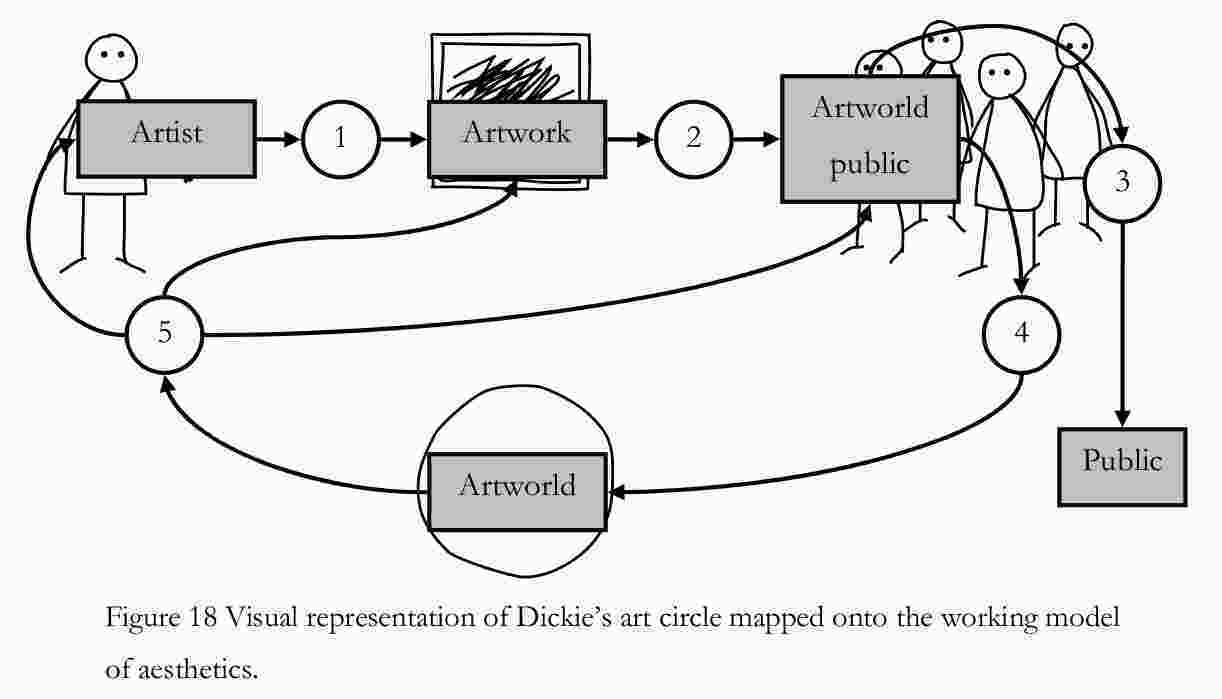
\includegraphics[width=\columnwidth]{./figures/artworld.jpg}

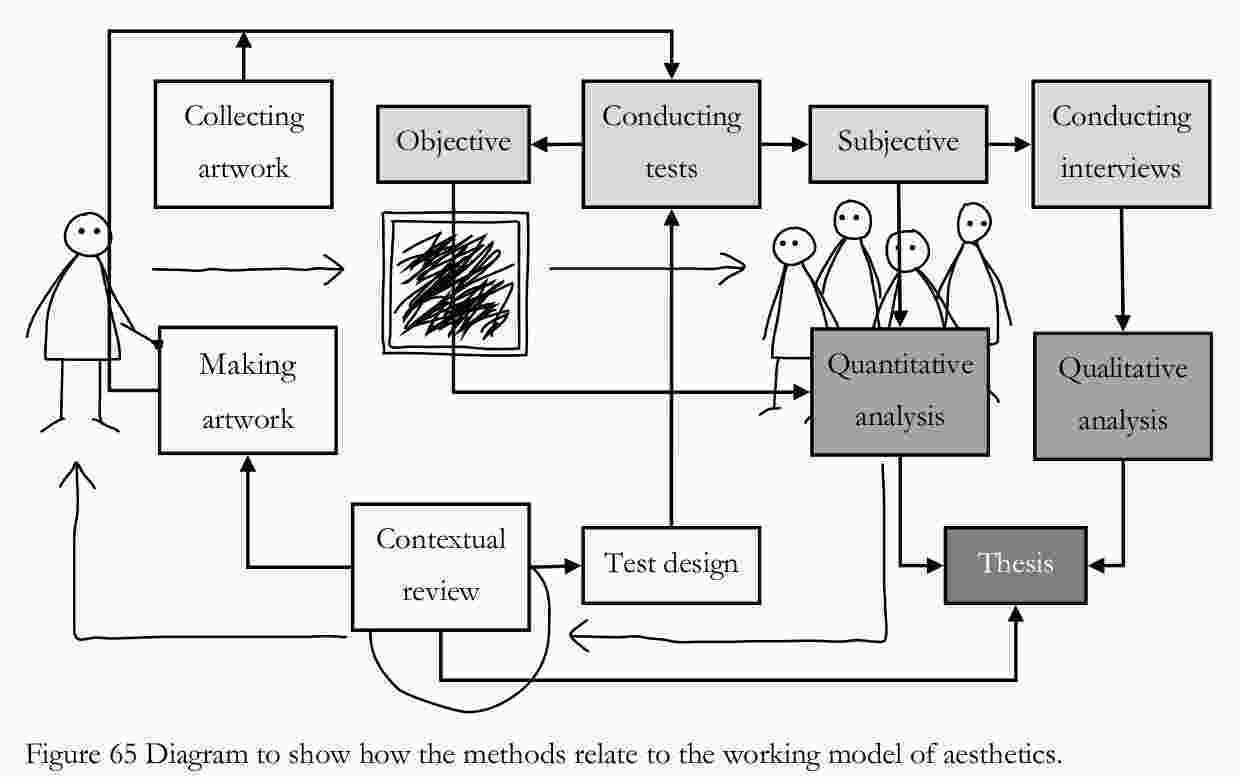
\includegraphics[width=\columnwidth]{./figures/aesthetic-research.jpg}

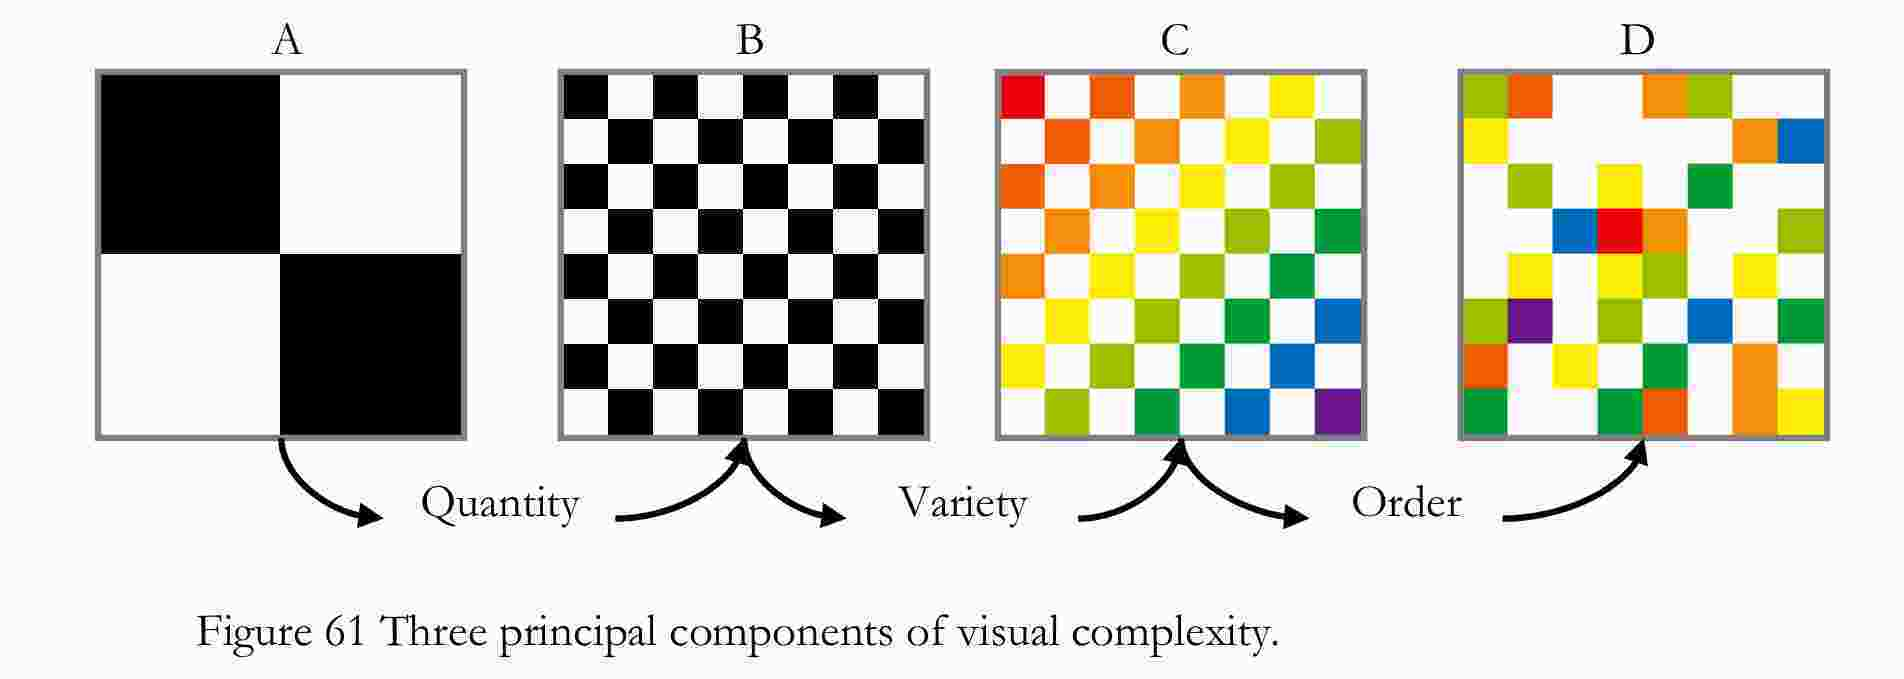
\includegraphics[width=\columnwidth]{./figures/quantity-variety-order.jpg}


%%COmment out 
%\bibliographystyle{apacite}
%\bibliography{./biblio}

%\end{document}

%% To the extent possible, exchanges of dialogue such as the example given in Section \ref{sec:writers-workshop} in the process language should be a
%% matter of dynamics rather than representation: this is another way to
%% say that ``triggers'' should be independent of their ``results.''
%% Someone saying something in the workshop does not cause the
%% participant to act, but rather, to think.
%% In order to facilitate this sort of interaction, it would be necessary
%% for systems to implement a basic protocol related to
%% %%
%% {\tt presentation}, {\tt listening}, {\tt
%%   feedback}, {\tt questions}, and {\tt
%%   reflections}.
%% %%

%% \begin{description}
%% \item[Presentation:] definition ***
%% \item[Listening:] definition ***
%% \item[Feedback:] definition ***
%% \item[Questions:] definition ***
%% \item[Reflections:] definition ***
%% \end{description}

% First attempt
%% Various social strategies, ranging from Writers Workshops to open
%% source software, pair programming, and design charettes have been
%% developed to exploit emergent effects and to develop new shared
%% language.  We investigate the feasibility of using designs of this
%% sort in multi-agent systems that learn by sharing and discussing
%% partial understandings.  Building on earlier theoretical work, we
%% describe concrete implementation plans and some preliminary results.
%%
%%
%%
% \item[] Research question: \emph{How do we implement feedback in
%  creative systems?}
